\documentclass[journal]{IEEEtran}
\IEEEoverridecommandlockouts
% The preceding line is only needed to identify funding in the first footnote. If that is unneeded, please comment it out.
\usepackage{cite}
\usepackage{amsmath,amssymb,amsfonts}
\usepackage{algorithmic}
\usepackage{graphicx}
\usepackage{textcomp}
\usepackage{balance}
\usepackage{xcolor}
%\usepackage{lipsum}
\usepackage{scalerel}
\usepackage{tikz}
\usetikzlibrary{svg.path}

\definecolor{orcidlogocol}{HTML}{A6CE39}
\tikzset{
	orcidlogo/.pic={
		\fill[orcidlogocol] svg{M256,128c0,70.7-57.3,128-128,128C57.3,256,0,198.7,0,128C0,57.3,57.3,0,128,0C198.7,0,256,57.3,256,128z};
		\fill[white] svg{M86.3,186.2H70.9V79.1h15.4v48.4V186.2z}
		svg{M108.9,79.1h41.6c39.6,0,57,28.3,57,53.6c0,27.5-21.5,53.6-56.8,53.6h-41.8V79.1z M124.3,172.4h24.5c34.9,0,42.9-26.5,42.9-39.7c0-21.5-13.7-39.7-43.7-39.7h-23.7V172.4z}
		svg{M88.7,56.8c0,5.5-4.5,10.1-10.1,10.1c-5.6,0-10.1-4.6-10.1-10.1c0-5.6,4.5-10.1,10.1-10.1C84.2,46.7,88.7,51.3,88.7,56.8z};
	}
}

\newcommand\orcidicon[1]{\href{https://orcid.org/#1}{\mbox{\scalerel*{
				
\begin{tikzpicture}[yscale=-1,transform shape]
					\pic{orcidlogo};
				\end{tikzpicture}
			}{|}}}}

\usepackage{hyperref} %<--- Load after everything else

\def\BibTeX{{\rm B\kern-.05em{\sc i\kern-.025em b}\kern-.08em
		T\kern-.1667em\lower.7ex\hbox{E}\kern-.125emX}}
\newcommand{\linebreakand}{%
\end{@IEEEauthorhalign}
\hfill\mbox{}\par
\mbox{}\hfill\begin{@IEEEauthorhalign}
}

\begin{document}
\title{RFID Based Fruit Monitoring and Orchard Management System}
\author{B.~H. M.~Imdaad \orcidicon{0009-0003-0377-5055}, S.~I.~Jayalath \orcidicon{0009-0003-7056-8603}, P.~C.~G.~Mahiepala \orcidicon{0009-0006-9708-2488}, M.~K.~T.~Sampath \orcidicon{0009-0003-6823-9958},\\ and S.~R.~Munasinghe \orcidicon{0000-0003-3445-4767},~rohan@uom.lk,~\IEEEmembership{Senior Member,~IEEE}

\thanks{Manuscript received 4 October 2023; revised 12 December 2023, 9 February 2024, and 11 May 2024; accepted 12 May 2024. This work was non-monetarily supported by Nelna Agri (Pvt.) Ltd. This article was recommended by Associate Editor Luisa Petti.}
\thanks{B.~H. M.~Imdaad, S.~I.~Jayalath, P.~C.~G.~Mahiepala, T.~Sampath, and S.~R.~Munasinghe ORCID-0000-0003-3445-4767, email:~rohan@uom.lk are with the Department of Electronic and Telecommunication Engineering, University of Moratuwa, Moratuwa, 10400 Sri Lanka.}
\thanks{S.~R.~Munasinghe is a visiting fellow at the Department of Global Development, College of Agriculture and Life Sciences, Cornell University, Ithaca, NY 14850, USA.}
\thanks{Digital Object Identifier 10.1109/TAFE.2024.3402710}}

\markboth{IEEE Transactions on Agrifood Electronics, Vol.~00,~No.~0,~2024}
{Shell \MakeLowercase{\textit{et al.}}: Bare Demo of IEEEtran.cls for IEEE Journals}

\maketitle
\begin{abstract}
	This research presents an efficient fruit monitoring and orchard management system to replace the existing paper-based manual process. The new method is based on five state-of-the-art technologies, namely Radio Frequency IDentification (RFID), Wi-Fi network, Mobile App, Coud database/server, and Web Application. This paper presents the proper integration of these technologies to provide an effective, worker-friendly, and cost-effective solution to the problem. The proposed method starts by attaching RFID tags to each tree and each fruit and registering them in the cloud database. The cloud server visualizes the status of the orchard and implements inventory management. Workers use a hand device for tasks such as bagging, spraying, and plucking. The orchard manager carries out task assignments and worker deployment on the web application. Each worker gets notified of the assigned tasks on his field device, and when such tasks are accomplished, the status is updated in the cloud database. Using this system, each fruit is monitored from the initial covering state to the final plucking state. On the contrary, the existing paper-based manual process suffers from improper spraying that leads to disease-spreading infestations and loss of yield. Due to the existing inefficiencies  the price of fruit has gone up to a limit that is not affordable to the public, hence unprofitable to the grower as well. In this context, the proposed solution will help monitor and manage fruit orchards efficiently, which will increase the quality and quantity of the yield while lowering the cost of production. 
\end{abstract}
\begin{IEEEkeywords}
Fruit inventory management, Fruit monitoring, Handheld Radio Frequency Identification (RFID), Internet of Things (IoT).
\end{IEEEkeywords}
\section{Introduction}
Smart monitoring and management of fruit orchards are critically important to high-quality yield and lower cost of production. In \cite{apple}, Wu et. al. present a fruit monitoring and management system for an apple orchard in which the production process is monitored to reduce the time and labor. This research also uses RFID technology \cite{RFID} to identify fruit trees and to monitor the spraying of agrochemicals and fertilizers. Behera et. al. \cite{behera2021tree} proposes a method to monitor fruits in trees using sensors and  Internet of Things (IoT) technology in that fruit status and environmental conditions are monitored using cameras and sensors. The cameras used are solar-powered and they are Wi-Fi connected for remote viewing for farm management. Rain sensors, temperature sensors, and moisture sensors are deployed to access the environmental information. This method requires infrastructure development over the entire orchard, which makes it costly and difficult to scale for commercial deployment. The EU Horizon project \cite{EU2020} proposes a method based on artificial intelligence to accurately count apples with the size that will help growers to know the harvest with higher accuracy. Several high-tech solutions including sensor networks \cite{Yuan}, drones \cite{Suryawansi}, robots \cite{Mengoli}, and LiDaR \cite{Tsoulias}, have been tested for orchard management and fruit monitoring, however much of it is not scalable and cost-effective for commercial deployment. Hence, there is a need for a cost-effective, and scalable solution for fruit monitoring in large orchards. In this context, this research proposes a novel technique for on-tree fruit monitoring and orchard operation scheduling. The method is custom-designed for mangoes to improve the quality of yield and reduce the cost of operations (bagging, spraying, and plucking). It also helps reduce the loss of yield due to pest attacks and ill-treatment. The method was designed by proper integration of state-of-the-art technologies \cite{Ruiz}, \cite{architecture}.\par
The proposed solution requires RFID tags attached to each fruit and each tree. Once scanned, the fruit and tree information are sent to the cloud server/database. The web application visualizes the orchard status for the agronomist to schedule tasks and assign workers. The scheduled tasks are communicated to the hand devices of the workers. As the workers perform the scheduled tasks the orchard status is updated concurrently while issuing flags if the task is not performed as scheduled. This way, timely fruit treatment, high-quality yield, and efficient labor deployment can be guaranteed. The RFID tags are reusable because they are protected inside the translucent bags. The hand device component cost is only \$25, and only about fifty such devices are needed even for a large orchard because the workers are deployed in small teams of six to ten workers. Due to the same reason, the proposed solution can be implemented in a large orchard quite easily by deploying as many small worker groups as needed. This does not require any scale-dependent modifications to the solution because worker groups operate independently. The functionality of the proposed system was verified through a field test.
\section{Mango Orchard Management}
In mango orchards, where the Tom EJC mango variety shown in Fig.\ref{fig_TomEJC} is grown, the first activity is "bagging", in which each fruit at the size of a chicken-eg is placed inside a translucent bag to protect them from pests. The bag also helps the fruit get a bright yellow color. For the rest of the season, until plucking the fruits remain inside these bags as shown in Fig.\ref{fig_TomEJC}.
\begin{figure}[h]
	\centering
	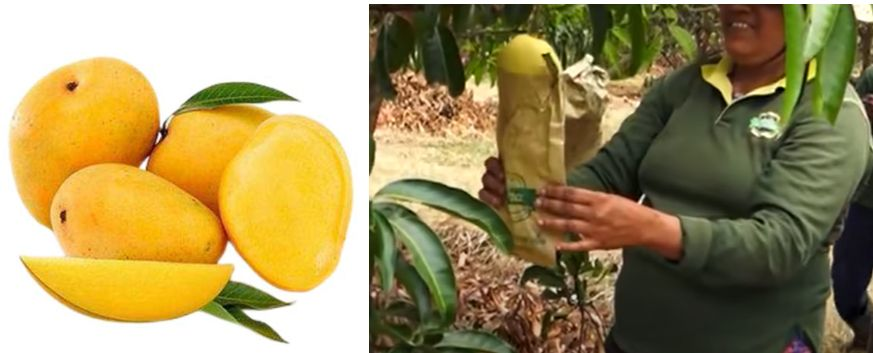
\includegraphics[width = 8.5cm]{graphics/TomEJC.png}
	\caption{Tom EJC mango covered in a carbon-coated protective bag. Photo from Nelna Agri website}
	\label{fig_TomEJC}
\end{figure}
The existing practice is manual "bagging" in that a worker records on paper each tree and the number of fruits it bears. The same information is written on the outer surface of each bag. A few times within the season, workers are deployed to spray antifungal chemicals onto the fruits for that the workers have to read the date information on each bag, open the relevant bags of respective age, and spray the chemicals. After about seventy-five days, workers open the bags, inspect the maturity, and pluck the mature fruits. Premature fruits are kept in the bag for a few more days. The ad-hoc task assignment and worker deployment in the present practice reduces worker efficiency and increases the cost of production. There are about fifty thousand mango trees in the orchard, and in one season, nearly around a million mangos are plucked. Given the scale, even a marginal improvement to the existing practice will result in a significant return on investment.
\section{Proposed Fruit Monitoring and Orchard Management System}
Figure \ref{fig_system} shows the block diagram of the proposed solution. This system consists of the following five components, labeled A, B, C, D, and E in Fig.\ref{fig_system}.
\begin{itemize}
	\item[] A - Hand device with RFID reader
	\item[] B - Local Wi-Fi mesh network in group deployment
	\item[] C - Mobile application
	\item[] D - Cloud server/database
	\item[] E - Web Application
\end{itemize}
\subsection{Hand Device}
\begin{figure}[]
	\centering
	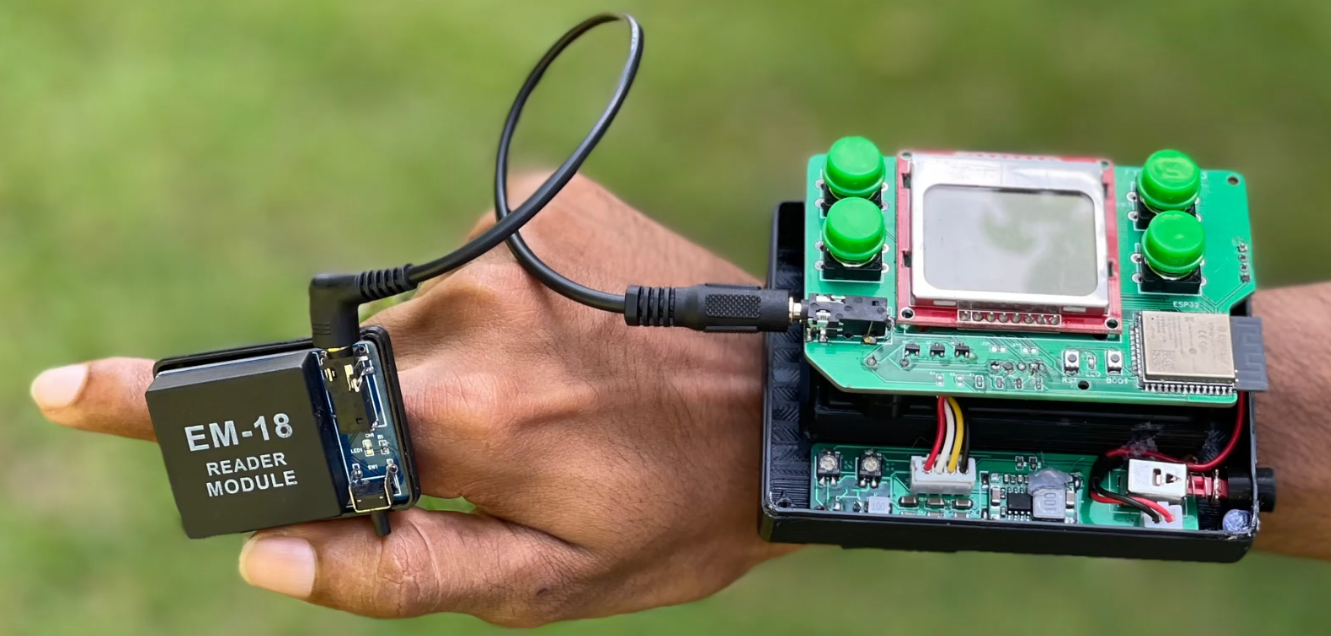
\includegraphics[width = 8cm]{graphics/handheld.png}
	\caption{Handheld unit with RFID scanner}
	\label{fig_handheld}
\end{figure}
\begin{figure*}
	\centering
	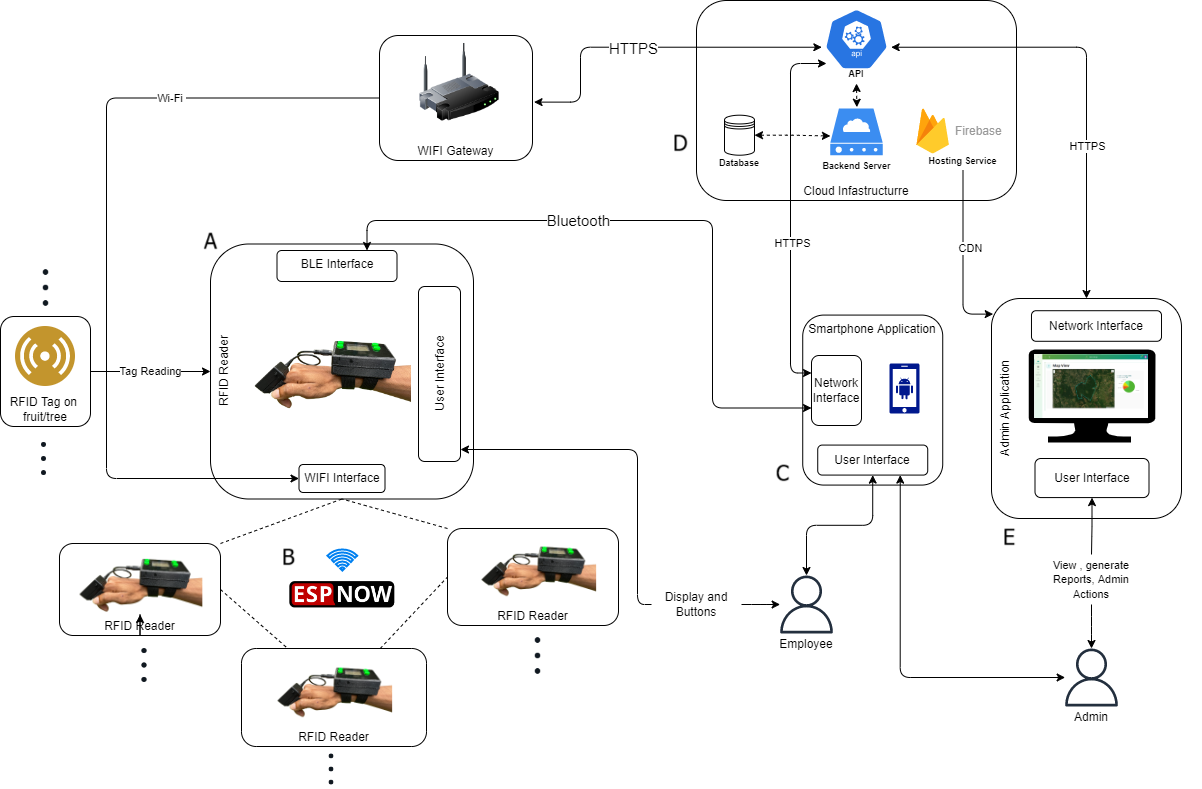
\includegraphics[width = 17cm]{graphics/system.png}
	\caption{System design: A-Field device with RFID reader, B - Mesh network of field devices in group deployment, C - Mobile application, D - Cloud server/database, E - GUI (Graphical user interface)}
	\label{fig_system}
\end{figure*}
Fig.\ref{fig_handheld} shows the hand device. The workers receive their assigned tasks to their respective hand devices and when they perform the tasks as a group, the hand devices share the group data among themselves through the local Wi-Fi mesh network. This device has a 5cm ranged 13.56MHz RFID reader \cite{rfid_1356Mz}, a Wi-Fi module, a Bluetooth module, a Nokia 5110 display, a keypad, a power supply, and a system-on-chip (SoC). The field device consists of three printed circuit boards (PCB) for the power system, main functionality, and the RFID module. The power supply PCB provides 5V and 3.3V to the main PCB and RFID module. The main PCB was designed with an ESP32 microcontroller with C language-based firmware controls. The FreeRTOS operating System \cite{rtos} was used to develop the firmware. The following functionalities are implemented in the firmware.
\begin{itemize}
\item \textbf{Communication with the server} - The reader device communicates with the server through Wi-Fi, and receives the tasks assigned.
\item \textbf{Communication between field devices} - Field devices communicate through the mesh network and synchronize data of the task being implemented.
\item \textbf{Instructions to the Worker} - The device shows the worker the assigned tasks with the block and sub-block information, guides the worker to perform the task, audits the worker, and notifies if a certain task is missed.
\end{itemize}
	The hand device is powered with two serialized 3.7V Li-ion 18650 3000mAh batteries. Nominal current is measured as 85mA, which sets the operational duration of the device to 21 hrs, or minimally three days with a single charge \cite{power}. The component cost per field device is approximately \$25, which includes the cost for ESP32, Battery, 84x84 LCD 5110 Nokia, PCB, Enclosure, and the RFID Reader. Almost all functions of the hand device could be implemented with a modern smartphone with a built-in RFID reader. However, this option was eliminated due to the following reasons.
	\begin{itemize}
		\item Agrochemical spraying while handling a smartphone requires both hands of the worker, which is very inconvenient. A wearable device, on the other hand, is more convenient.
		\item Smartphones are not designed to cope with the rough field conditions like a mango orchard where agro-chemicals are used nearby.
		\item Utilizing smartphones is associated with the risk of leaking confidential data out of the grower.
		\item The workers generally don't have modern smartphones with the RFID reading. And, it's not cost-effective for the grower to provide modern smartphones while the hand-wearable device costs only \$25.
	\end{itemize}
\subsection{Wi-Fi Mesh Network of Hand Devices}
A few groups of six to ten workers are deployed with hand devices for assigned tasks. The hand devices create a mesh network to exchange information within the group in real-time so that when a certain fruit is treated by one worker it is immediately known by other field devices in the group. The mesh network helps avoid situations such as two workers attempting to spray on the same fruit at two instants. The mesh network also enables temporary redundant data storage until data gets uploaded to the cloud database through the mobile network. This feature is crucial for orchards where mobile connectivity is not reliable. The Wi-Fi mesh network is created using ESPNow \cite{ESPNow}, and the communication between field devices is maintained using the inbuilt BLE and Wi-Fi.\par
After comparing available options such as the Wi-Fi mesh, the Bluetooth mesh, and ESP-now mesh, the latter was chosen as the most appropriate mesh network due to low power consumption, ease of implementation, and cost-effectiveness \cite{7566486}. ESPnow establishes a 15-20m range mesh network that is quite appropriate for this application. The ESP module in the hand device has required hardware built-in to support ESPNow protocol.
\subsection{Mobile App}
Fig.\ref{fig_app} shows the two pages of the mobile app.
\begin{figure}[htb]
	\centering
	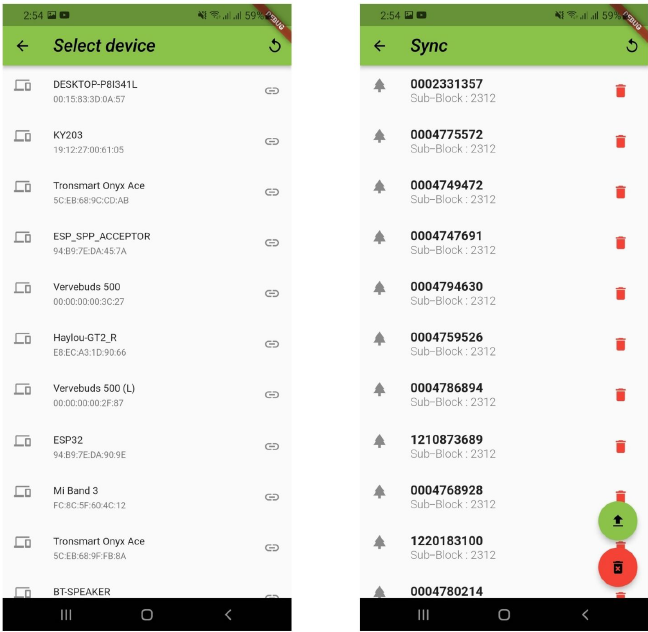
\includegraphics[width = 8cm]{graphics/app.png}
	\caption{Mobile app: Left - the nearby field devices for the worker to select his device, Right - worker selects the collected data to be sent to the cloud database}
	\label{fig_app}
\end{figure}
Workers carry the mobile app with them only once, during the registration of trees and fruits. The mobile app connects to the hand device of the worker through Bluetooth. When the worker scans an RFID tag, the ID is fetched to the mobile app where it is added with the GPS (Global Positioning System) information, block number, and sub-block number. The mango orchard is divided into larger blocks, and each block is divided into sub-blocks.
And, when the worker adds the tree to the cloud database, he sets the block number and sub-block number on the field device, and then scan the RFID attached to the tree. When fruits are registered, the worker has to first scan the tree RFID, and then the fruit RFIDs to associate fruits belonging to a tree. The mobile App communicates with the cloud server through an API, and it communicates with the field device through Bluetooth. The mobile app was developed using Flask, a Python-based microframework for mobile application development.
\subsection{Cloud Server and Database}
The cloud server exposes APIs and maintains communication with hand devices, admin applications, and mobile applications using JWT token-based authentication. The functions of the cloud server are as follows:
\begin{itemize}
	\item Registering and authenticating field devices and workers.
	\item Providing geographical data, employee data, fruit, and tree data, and reports to the web application.
	\item Exposing APIs to collect the following information from the reader devices and mobile applications.
	\begin{itemize}
		\item New fruits
		\item Fruits pending spraying
		\item Fruits sprayed on time
		\item Plucked fruits
		\item Fallen/Missing fruits
	\end{itemize}
\end{itemize}
The cloud server was developed as a Java Springboot application. A MongoDB \cite{gyHorodi2015comparative} database which is connected to the cloud server stores information about fruits, tasks, and status maps.
\subsection{Web Application and GUI}
The web application is used for the following tasks:
\begin{itemize}
	\item Orchard information such as the block, sub-block, and worker details can be entered into the system.
	\item Tasks can be assigned to the workers.
	\item Visualize the map giving an overview of the orchard status, allowing the grower to navigate and view the details.
	\item Generates reports about the progress and employee performance.
\end{itemize}
The web application visualises orchard status by pulling block, sub-block, tree ID, and fruit IDs from the cloud database. The grower can visualize the status of the orchard on the GUI as illustrated in Fig.\ref{fig_status}, which shows the status of a sub-block at a given time. It indicates that there are four trees in the sub-block, and one mango is "bagged", one mango has got $SPRAY\_1$, one mango has got $SPRAY\_2$, four out of five mangos have been plucked, and one mango is missing.
\begin{figure}[h]
	\centering
	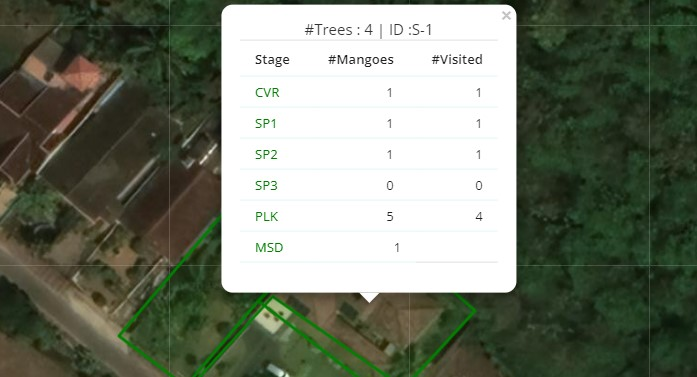
\includegraphics[width = 8.5cm]{graphics/map.jpg}
	\caption{Status of a sub block. There are five blocks and fourty sub-blocks. Each sub-block has about thousand mango trees.}
	\label{fig_status}
\end{figure}
The tasks can be scheduled using the web application.
Figure \ref{fig_1}(a) shows how $worker\_01$ is assigned to spray twenty mangos in ten trees, and Fig. \ref{fig_1}(b) shows the assignment of $worker\_1$ to pluck twenty mangos in ten trees. Once these assignments are scheduled, the same information appears in the field device of the $worker\_01$.
\begin{figure}[h]
	\centering
	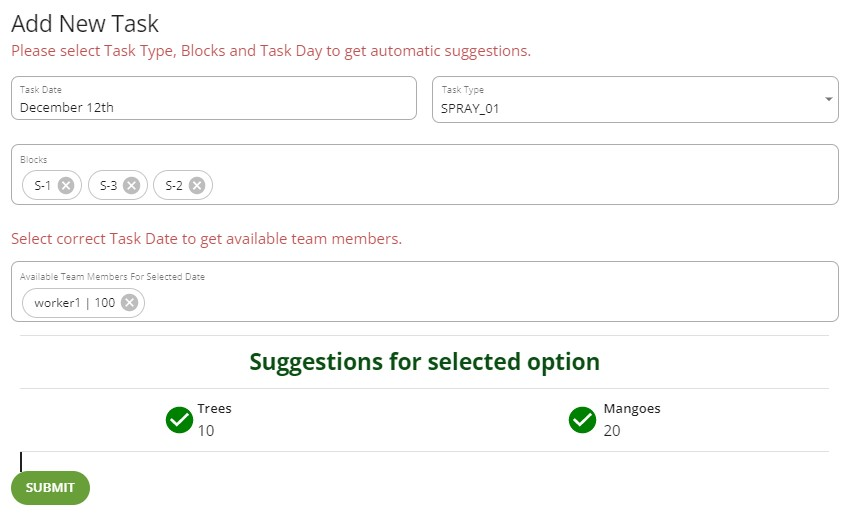
\includegraphics[width = 8cm]{graphics/1a.jpg}(a)\\
	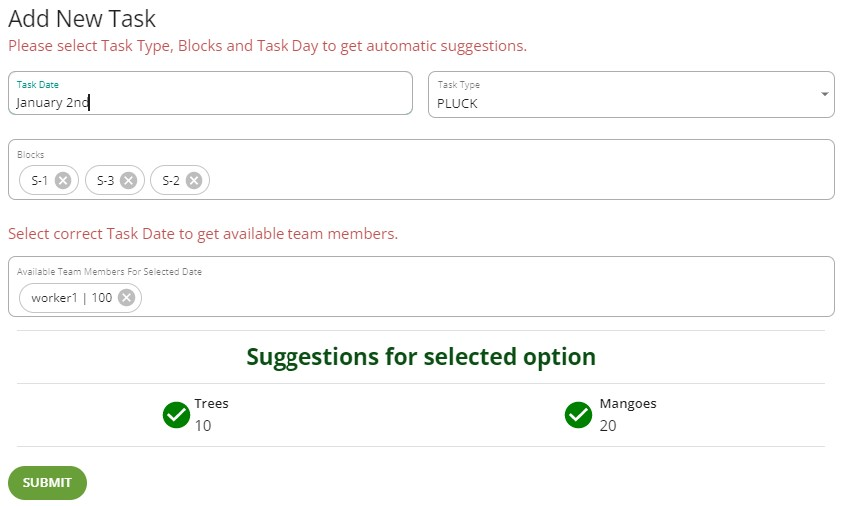
\includegraphics[width = 8cm]{graphics/1b.jpg}(b)
	\caption{The scheduling of a spraying task and a plucking task, and assigning it to a worker using web application}
	\label{fig_1}
\end{figure}\par
Fig.\ref{fig_GUI} shows the summary of two assigned tasks; covering, and spray\_1.
\begin{figure}[htb]
	\centering
	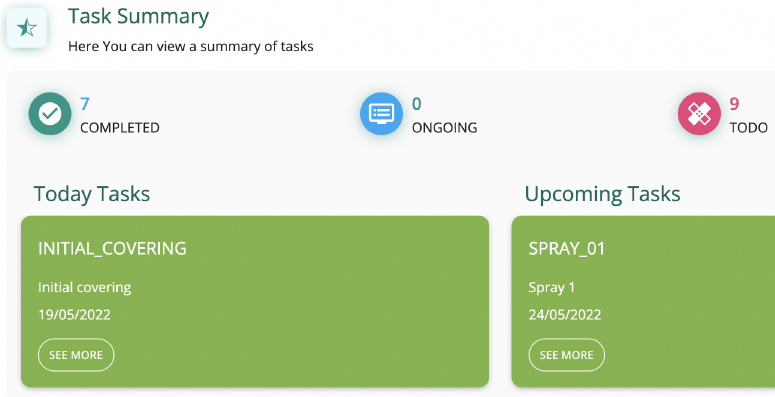
\includegraphics[width = 8.5cm]{graphics/GUI.png}
	\caption{GUI indicating the task summary: seven tasks have been completed and 9 tasks are to be carried out}
	\label{fig_GUI}
\end{figure}
The web application was created using ReactJS, which is a free and open-source front-end JavaScript library \cite{webVsDesk}. The application communicates with the cloud server via REST APIs and is authenticated with JWT (JSON Web Token) \cite{jones2015json}. The information is stored in the redux store, the central bucket which stores all the states of the admin web application. 
The GUI is hosted in a cloud hosting service, hence, it can be accessed from anywhere to perform orchard monitoring and schedule tasks. The GUI communicates with the cloud server via an API.
\section{Field Test}
The fruit treatment process is implemented by small worker groups of six to ten. A few such groups are deployed daily, and these groups operate independently. Hence, the proposed solution can be implemented independently of the scale of the orchard if it properly functions within a single worker group. For a large orchard, only the cloud server capacity and communication bandwidth need to be scaled to handle the data coming from the worker groups concurrently. On the other hand, the worker group devices re-attempt and get the data uploaded to the server ubiquitously in situations of high data rates. Therefore, a small-scale field test was implemented to test and verify the effectiveness of the proposed solution within a single worker group. A few units were built for the field test.\par
Figure. \ref{fig_3} compares the result of the existing practice and the proposed method. All mangoes were bagged on Day$\_$0, Spray$\_$1 was carried out on Day$\_$20, Spray$\_$2 was carried out on Day$\_$40, and mangoes were plucked on Day$\_$70. As shown in Fig. \ref{fig_3}(a) the worker missed Spray$\_$1 on nineteen mangoes on Day$\_$20, which was corrected by the hand device as shown in Fig. \ref{fig_3}(b). Again, on Day$\_$40, there were ten mangoes without receiving a single spray, and there were twelve mangoes with only one spray as shown in Fig.\ref{fig_3}(a), However, the hand device notification in the new system guided the worker not to miss even a single mango as shown in Fig.\ref{fig_3}(b). The outcome of the field test can be summarized as follows:
\begin{itemize}
	\item The proposed method increases the well-treated mangoes to 215/227, which is a significant $(94.7\%)$ improvement compared with the 190/227 mangoes, which is $(83.7\%)$ of the existing practice.
	\item The proposed method reduces the ill-treated mangoes to zero, whereas the existing practice records about 25/227, which is $11\%$ low quality mangoes due to missing sprays.
	\item The proposed method allows workers to enter missing and fallen fruits into the system separately. Workers observe missing and fallen mangoes during spraying and plucking. The existing practice does not have a proper way to record this information.
\end{itemize}
The existing practice does not provide accurate information about missing and fallen fruits separately. The proposed method provides exact numbers of missing and fallen fruits and allows the grower to take appropriate actions. For example, if a significant number of fruits go missing, the grower needs to tighten security measures. On the other hand, if there are too many fallen fruits, then the grower has to look into the chemical treatments.\par
Considering the additional cost of production, the grower prescribed only four scans for the field test. However, in actual implementation, more fruit scans could be implemented say on Day$\_$50, Day$\_$60, and so on to get a closer look at the process.
\begin{figure*}[ht]
	\centering
	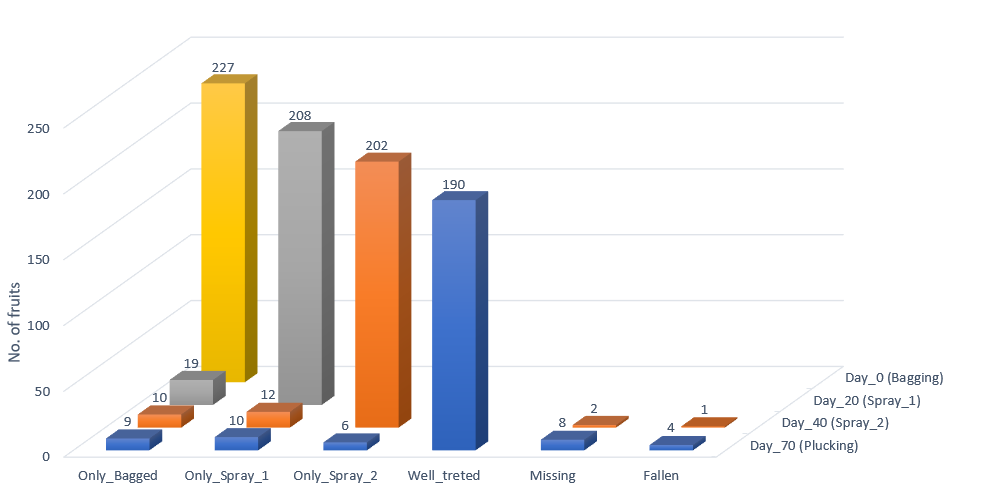
\includegraphics[width = 14cm]{graphics/Res_Old2}(a)
	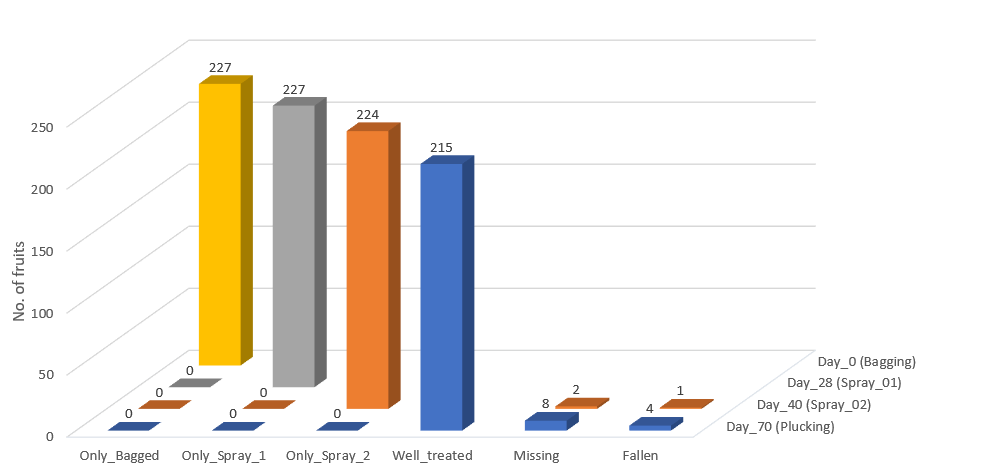
\includegraphics[width = 14cm]{graphics/Res_New2}(b)
	\caption{Typical result of the existing practice (a), and the actual result of the proposed method(b)}
	\label{fig_3}
\end{figure*}

\subsection{Fallen and Missing Fruits}
Fallen fruits are the fruits workers find on the ground with the bag used for initial covering. The worker scans the RFID of the fallen fruit and registers it as “fallen”. The missing fruits are nowhere to be found, and only the hand device can detect it when the workers walk from the present tree to the next. The hand device then indicates that there is another untreated fruit in the present tree, but the workers cannot find it. Then, a worker has to register the fruit on the hand device as “missing”
\section{Conclusion}
A smart solution for fruit monitoring and orchard task scheduling has been designed, prototyped, and field tested. The proposed solution has a hand device with an RFID scanner, a local WiFi mesh network, a cloud server/database, a mobile application, and a web application. On the web application, tasks such as fruit bagging, spraying, and plucking are scheduled and assigned to workers at specific times of the season. The workers get notified of the assigned tasks on their hand devices, and they carry out the tasks using their hand devices. The data from the hand devices are fetched to the cloud database for concurrent orchard status updates.\par
In small worker group deployment, once a fruit is treated by a worker, all of the workers in the group get their information updated through the local WiFi mesh network. This eliminates workers approaching an already treated fruit, or leaving fruits without treatment. Hence, the proposed solution maintains accuracy and effectiveness in fruit treatment and worker deployment, which improves the quality and quantity of yield, and productivity of the workers. Small worker group deployment makes the proposed solution extremely cost-effective and deployable independent of the scale of the orchard. The proposed solution, though customized to mango, could be modified to other similar fruits.
The functionality of the proposed method was verified through a field test in which the entire process was tested end-to-end. It was verified that the proposed solution is highly cost-effective, technically feasible, and deployable independent of the scale of the orchard. The component cost per field device was just \$25 and even for a large orchard, only about fifty field units are required in small worker group deployment. In addition, cloud database subscription (\$75/year), mobile data charge (\$100/year), and one-time software development costs (\$1600) are involved. The system was designed for mango, however, it could be customized to other fruits of a similar nature.
\section{Acknowledgement}
This project was non-monetarily supported by Nelna Agri (Pvt.) Ltd, Sri Lanka. The authors acknowledge the valuable support from Prof. Lori Leonard, Prof. Ronnie Coffman, and Prof. Richard Cahoon of the Department of Global Development, CALS, and the AgriTech faculty of Cornell University, USA.
\balance
\begin{thebibliography}{1}
\bibitem{apple}
C.~Wu, H.~Zhang, J.~Zhang, W.~Tian, and H.~Cheng, ``An orchard management system with rfid-based apple tree identify detection,'' in Fourth International Conference on Digital Manufacturing and Automation, pp.~180--184, 2013.
\bibitem{RFID}
“Explore RFID Basics | RFID Tracking and Inventory,” Available online: https://rfid4u.com/rfid-basics-resources/
\bibitem{behera2021tree}
S.~K. Behera, P.~K. Sethy, S.~K. Sahoo, S.~Panigrahi, and S.~C. Rajpoot, ``On-tree fruit monitoring system using iot and image analysis", Concurrent Engineering, vol.~29, no.~1, pp.~6--15, 2021.
\bibitem{EU2020}
“Artificial intelligence for yield estimations at fruit orchards | AGERPIX Project | Fact Sheet | H2020,” CORDIS | European Commission, 2020, online  https://cordis.europa.eu/project/id/888783
\bibitem{Yuan}
H.~Yang, B.~Kuang and A.~M.~Mouazen, "Wireless Sensor Network for Orchard Management," 2011 Third International Conference on Measuring Technology and Mechatronics Automation, Shanghai, China, 2011, pp. 1162-1165, doi: 10.1109/ICMTMA.2011.859.
\bibitem{Suryawansi}
S. Suryawanshi, T. Baraskar, K. Umbrani and A. Chitnis, "Using Drone Technology for Fruit Orchard Management and Waste Reduction," 2022 6th International Conference On Computing, Communication, Control And Automation (ICCUBEA, Pune, India, 2022, pp. 1-9, doi: 10.1109/ICCUBEA54992.2022.10010999.
\bibitem{Mengoli}
D. Mengoli, R. Tazzari and L. Marconi, "Autonomous Robotic Platform for Precision Orchard Management: Architecture and Software Perspective," 2020 IEEE Intl.  Workshop on Metrology for Agriculture and Forestry, pp. 303-308, Tento, Italy, 2020.
\bibitem{Tsoulias}
N. Tsoulias, G. Xanthopoulos, S. Fountas and M. Zude, "In-situ detection of apple fruit using a 2D LiDAR laser scanner," 2020 IEEE International Workshop on Metrology for Agriculture and Forestry (MetroAgriFor), Trento, Italy, 2020, pp. 278-282, doi: 10.1109/MetroAgriFor50201.2020.9277629.
\bibitem{Ruiz}
L.~Ruiz-Garcia and L.~Lunadei, ``The role of rfid in agriculture: Applications, limitations and challenges,'' {\em Computers and Electronics in Agriculture}, vol.~79, no.~1, pp.~42--50, 2011.
\bibitem{architecture}
P.~Pierleoni, R.~Concetti, A.~Belli, and L.~Palma, ``Amazon, google and
microsoft solutions for iot: Architectures and a performance comparison'', IEEE Access, vol.~8, pp.~5455--5470, 2020.
\bibitem{ESPNow}
M.~S.~Koushik, M.~Sirinivasan, R.`Lavanya, S.~Alfred, and S.~Setty, ``Design and development of wireless sensor network based data logger with esp-now protocol", in {\em 6th International Conference for Convergence in Technology (I2CT)}, pp.~1--5, 2021.
\bibitem{power}
D.~Rimpas and A.~Kiatipis, ``Charging strategy effect on lithium polymer battery capacity: A case study,'' vol.~11, pp.~107--118, 11 2020.
\bibitem{7566486}
K.~K.C, ``Wireless mesh network: A survey,'' in {\em 2016 International
Conference on Wireless Communications, Signal Processing and Networking (WiSPNET)}, pp.~1966--1970, 2016.
\bibitem{rtos}
M.-Y. Zhu, “Understanding FreeRTOS: A Requirement Analysis,” May 2011, doi: 10.13140/RG.2.2.12419.09767.
\bibitem{rfid_1356Mz}
V.~Cernatescu and M.~Vladescu, ``An implementation of a 13.56 mhz rfid
reader,'' in {\em 2014 IEEE 20th International Symposium for Design and
Technology in Electronic Packaging (SIITME)}, pp.~103--104, 2014.
\bibitem{webVsDesk}
P.~M.~Martin Löfberg, ``Web vs. standalone application'' http://www.diva-portal.org/smash/record.jsf?pid=diva23A828988\&dswid=7259, 2005.
\bibitem{jones2015json}
M.~B.~Jones, J.~Bradley, and N.~Sakimura, “JSON Web Token (JWT),” RFC 7519, Tech. Rep., May 2015, https://datatracker.ietf.org/doc/rfc7519/
\bibitem{gyHorodi2015comparative}
C.~Gy{\H{o}}r{\"o}di, R.~Gy{\H{o}}r{\"o}di, G.~Pecherle, and A.~Olah, ``A comparative study: Mongodb vs. mysql,'' in {\em 2015 13th International Conference on Engineering of Modern Electric Systems (EMES)}, pp.~1--6, IEEE, 2015.
\end{thebibliography}
\end{document}
